\documentclass{article}
\usepackage[utf8]{inputenc}
\usepackage[a4paper, total={17cm,21cm}]{geometry}
\usepackage{graphicx}
\usepackage[export]{adjustbox}
\usepackage{url}
\usepackage[nottoc]{tocbibind}

\title{Software development of visualization system}
\author{Rohullah Khorami \& Fredrik Kortetjärvi}

\begin{document}

\maketitle
\newpage
\tableofcontents
\newpage
\section{Introduction}
There is a tremendous need for a visualization system connected to the property system KNX. To operate and test a larger property is very time-consuming and the risk of missing a deviation is big, that is why there is a need for some kind of application to solve these issues and minimize the processing time. Tekniska Byrån have a project to implement an application that works on Windows and Dotnet. The application is going to be connected to KNX by a driver can be implemented in any high-level programming language that works with Dotnet.
\subsection{Purpose}
The intended application will ensure quality testing and requires the time required to test the system on different real estate significantly. The purpose is to develop an application from a foundation that connects to the property system (via existing driver) and listens to the traffic to log in and display it graphically.
\subsection{Requirements}
The work will result in a visualization application that...
\begin{itemize}
    \item loaded with a structured csv file
    \item automatically generates control objects with tagged lines in the csv file
    \item handles on / off control, Light value 0-100\%, Up / down and Stop / step for shutter control, Position 0-100\% for shutter control
    \item has a function for connection to the KNX installation via an existing and open driver
\end{itemize}
\section{Background}
Tekniska Byrån is working with the KNX system and in this section, the background and a short introduction about Tekniska Byrån and KNX will be explained.
\subsection{Existing Project}
The KNX Ultimate is a where close application to the virtualization application. The KNX ultimate is written in Node red, making it more web-based oriented, but its use is less individual testing in KNX systems. This is the application that's closest to the goal of virtualization of KNX systems. 
\subsection{Teknisk Byrån}
Tekniska Byrån is a consultant in the electricity industry with a focus on innovative solutions and smart technology. The company currently has 3 employees and has been active since 2000.The employees work with advice, description and design of electrical installations and as far as possible with property automation and mainly KNX. Within KNX, they conduct design, commissioning, support, training and take care of office functions for interest association KNX Sweden. In addition to this, they have also programmed certain hardware and software against the system. Tekniska Byrån has premises in Vetlanda and Linköping and has over the years had several interns and supervised a degree project.\cite{tekAbout} 






\subsubsection{Services}
Tekniska Byrån is active in the following areas:
\begin{itemize}
    \item Electrical design: Activities in the field of electrical engineering include installation/construction. They install electricity in houses, apartments, schools, offices, and more. They also work in electrical design, construction, and documentation.\cite{tekelproj} 
    \item Programming: Tekniska Byrån jobs have programming projects to be able to have 
    smart functions in their property system. Tekniska Byrån performs smart property automation with programming for
 KNX/EIB(ETS), IHC-Smart House, Mod-bus, PLC(Programmable Logic Controller), 
 SCADA(Supervisory Control and Data Acquisition), OPC(Open Platform Communication),
 and the programming languages are HTML, ASP, PHP, VB, SQL.\cite{tekprog} 
    \item Education: The technical agency has many completed education programs and also in real estate automation and CAD technology. Property automation training includes an introduction to intelligent properties, a complete certified education center for KNX and IHC-Smart House.\cite{tekut} 
\end{itemize}


\subsubsection{Products}
Building Portal Suite creates a portal to the KNX system in the form of a simple PC application. In the Application, different functions can be handled depending on which component is installed.
Products that Tekniska Byrån develops that are used for smart properties are the following:\cite{tekprod} 
\begin{itemize}
    \item Alarm: The alarm is a compact, easy-to-use, customizable and flexible program for Windows that displays and follows up alarms in the KNX system. The alarm takes care of 3 different alarm classes (A, B, and C) where class A has the highest priority and audio features are used to attract attention.\cite{tekalarm} 
    \item Controller: The user can with the included interface configure their buttons and display the data. The Controller is easy to use and customizable at the same time. The states and values displayed are actual values loaded from the system. All fields are updated automatically. Programs for the controller are flexible and compact for windows desktop.\cite{tekcontroller} 
    \item Logger: Logger collects measurement data from the KNX system. The data that the logger collects can be used for example debiting, analysis or visualization with the help of a diagram. All values are saved together with the date and time when they were read. The values can be easily exported to XML and imported into another application for example in Excel, for further processing.\cite{teklogger} 
    \item Meter: Meter is a flexible program for PC that collects measurement data from energy meters in the KNX system. The purpose of collecting energy measurement data is that they can be used for further processes like debiting, analysis or visualization with the help of a diagram. To save the data in this program is the same process as in the logger program.\cite{tekmeter} 
\end{itemize}



\subsection{What is KNX?}
KNX is known as the European Installation Bus (EIB). It is a building control communication system that uses information technology to connect devices such as sensors, actuators, controllers, operating terminals, and monitors. 
KNX was found in May 1999 by the European installation bus association (EIBA), European home systems association (EHSA), and BatiBus club international (BCI) associations.\cite{KNXLegacy}\cite{Automation} \\

KNX is an open global standard for commercial and domestic building automation. KNX is ISO/IEC
14543-3. This standard is based on open systems interconnection(OSI)\cite{alma991000857549505936}, ISO/IEC 14543-3 is a
wireless protocol for low power devices. The protocol is made to keep switches and sensors super
low energy consumption. KNX is built upon the predecessor European installation bus
(EIB) and is compatible with every EIB compatible devices.   
KNX standard is extended from an OSI-based protocol stack with the physical layer. \cite{iso}\cite{Automation}.
 \subsubsection{Why KNX?}
 Smart homes technology improving fast and KNX has already had the latest technologies such as the internet of things in their current software. KNX plays a huge role in building automation (Smart House) worldwide and here are some reasons why KNX is important to learn: 
KNX provides the ideal introduction to the world of bus technology a lot of new functions and features are used in KNX current bus systems for example bit rate, media access control, data frames, and protocols. Learning KNX helps to become familiar with how to solve automation-related problems. There are 10\% of electronic industries that can plan and install KNX systems.\cite{KNXBenefits}\cite{Automation} \\

KNX's mission is to work with automated homes. KNX is working on automation technologies that the smart home market recognizes KNX association, But what is an automated home?\\
The automated home is also known as a smart house. Automated homes incorporate common devices that control features of the home. In the beginning, the functionality of a smart home was to control environmental systems such as lighting and heating, but technology has been developed so that every electrical component within the house can be included in the system. By smart house means that all electrical devices work together and can modify by smartphones or by an application that is connected to a network. Devices communicate with each other by using the "busline". A busline is a cable that connects all the devices and enables inter-connectivity between devices in different rooms throughout the home. \cite{SETAG}\cite{Automation} \cite{TheAdaptiveHouse}
\subsubsection{KNX Bus Devices}
KNX devices can be classified into four main groups like in Figure \ref{fig:knx}\cite{Automation}: 
\begin{itemize}
    \item System components(Power supply units, accumulators, USB interfaces, and more).
    \item Sensors(Switch sensors, motion detectors, and glass break detectors).
    \item Actuators(Switch and blinds).
    \item Logical components and control panel. 
\end{itemize}  
\begin{figure}[h!]
    \centering
    \includegraphics[width=8cm, height=8cm]{KNX.png}
    \caption{Devices over KNX}
    \label{fig:knx}
\end{figure}
To connect these devices the following communication media are available for a KNX system.\cite{KNXBasic} 
\begin{itemize}
    \item KNX twisted pair(KNX TP): The twisted pair is a cable with two twisted conductors for a single circuit 
    for enhancing electromagnetic compatibility (EMC) that will be acceptable
    in the electromagnetic environment.\cite{fdaEMC}
    \item KNX power line(KNX PL): Using the electricity cables in a building as a communication medium. 230V main electricity will provide the power required by bus devices.
    \item KNX radio frequency(KNX RF): Communication with the help of radio signals.
    \item KNX Ethernet(KNX IP): Communication with the help of internet protocols.
\end{itemize}
\newpage
\subsubsection{KNX Telegram}
KNX bus devices exchanges data between each other by telegram. A telegram consists of 8 bits characters, and a field is a combination of several characters. The communication media have different telegram structures\cite{KNXBasic}:
\begin{enumerate}
    \item KNX Twisted pair telegram has four fields: 
    \begin{itemize}
        \item Control field: It is responsible for receiving a response from the receiver whether the telegram transmission was successful or not. 
        \item Address field: This field contains the address of the sender and receiver.
        \item Data field: This field contains the telegrams payload.
        \item Checksum: It field is for parity checks. By parity check means that this field is used for detecting errors in the communication channel. \cite{KNXBasic}
    \end{itemize}
    \item KNX Power line has four fields: 
    \begin{itemize}
        \item Training field: This field arranges and sets the levels of senders and destinations. 
        \item Preamble field: The objective of this field is to show the start of transmission, control access to the bus, and avoids telegram from a collision.
        \item Third field: This field contains the KNX twisted-pair telegram. 
        \item System ID field: This field keeps an ID of signal from different KNX power line systems separately. It is because devices with the same ID can communicate with one another.\cite{KNXBasic}
    \end{itemize}
    \item Radio Frequency telegram 
    \begin{figure}[h!]
        \centering
        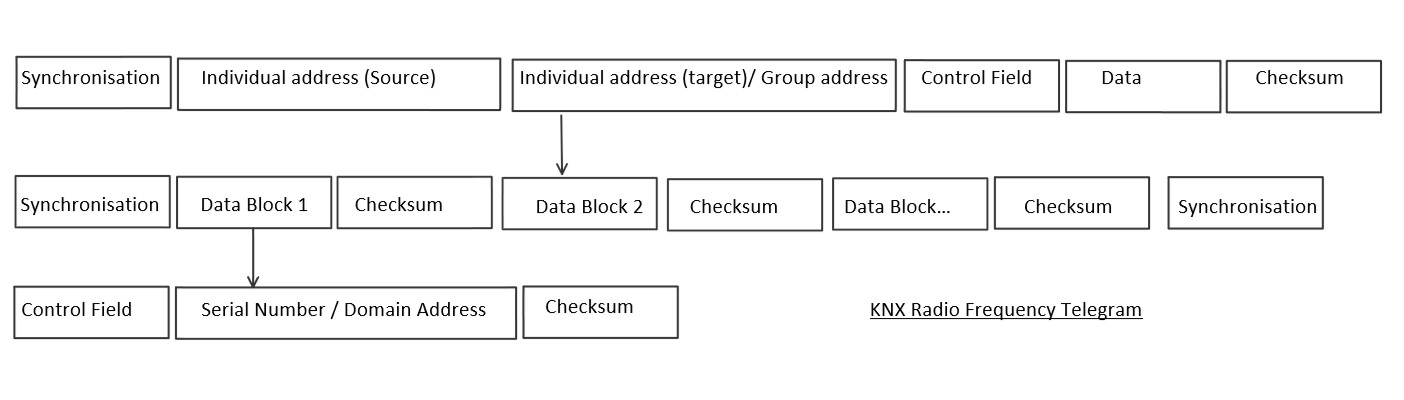
\includegraphics[width=\textwidth]{RF.jpg}
        \caption{Radio Frequency \cite{KNXBasic}}
        \label{fig:my_label}
    \end{figure}
    \item KNX internet protocol telegram
    \begin{itemize}
        \item Header Length: This field is to identify the stat of the telegram. 
        \item Protocol version: This field shows what version of the KNX IP applies. 
        \item KNX IP service type identifier: It shows the action that should be carried out.
        \item Total length: The objective of this field is to show the size of the KNX IP telegram.
        \item KNX IP body: this field contains telegrams payload. \cite{KNXBasic}
    \end{itemize}
\end{enumerate}
\section{Method}
\subsection{Tests}
The test will ensure that the application is working like intended and follow the requirements from the company. 
\subsubsection{Driver test}
Driver test will check if the application can communicate with the KNX devices like intended.  The test will check if the application is connecting to the bus system and ensure that the baseline settings will give back the expected result. The driver will be tested against hardware that the company will provide. 
\subsubsection{Design test}
The design test will test the design on the application with design case techniques. These techniques do a width 
range of tests that will get a width coverage. The tests that will cover the design part are error 
guessing, equivalence partitioning, boundary value analysis, decision table technique, and state transition technique.\\

Error guessing is a technique to guess what the user could do to give back an error. This technique aims to find the human error from a person who has not programmed the application and knows what's right. The example, we have a text box, and we programmer knows only numbers that work in the box, but users can write whatever they feel like no one can say what's wrong or guide them. They could write text instead of numbers.\\

Equivalence partitioning is a class case test where a significant interval is divided into classes. There 1 level; get one test each and then see if the level passes. The Equivalence partitioning tries to minimize the trials but still has good coverage over the whole interval. For example, if we have an interval between 1-200, it's too many tests if we take from 1-200 one by one.
Instead, we divide the interval into classes like -101 $\rightarrow$ 0, 1 $\rightarrow$ 100,\\101 $\rightarrow$ 200, and 201 $\rightarrow$ 300 and test every case if its passes. From every class, you choose one value to test, and if that passes, then the whole class passes.\\

The boundary value analysis technique finds weaknesses in the boundary values. It takes the matters and test right before it and right inside the value and the value this ensure that the boundary works like intended.\\

The decision table technique checks for failures in the application's conditions and how many to test is two power of numbers of cases. For example, the application has three conditions. Then it will be two power of 3, and that's 8. so we have a whole eight tests for three conditions. \\
Example:\\ 
Condition 1: person over 40 = 15\%\\
Condition 2: person under 40 = 10\%\\
Condition 3: person with coupon = 30\%\\
\begin{table}[h!]
    \centering
    \begin{tabular}{c|c|c|c|c|c|c|c|c|}
        &Rule 1&Rule 2&Rule 3&Rule 4&Rule 5&Rule 6&Rule 7&Rule 8  \\
        Condition 1&T&T&T&T&F&F&F&F\\
        Condition 2&T&T&F&F&T&T&F&F\\
        Condition 3&T&F&T&F&T&F&T&F\\
        Result&X&X&45\%&15\%&40\%&10\%&X&X\\
        
    \end{tabular}
    \caption{Example}
    \label{tab:my_label}
\end{table}
Every column will be a test to test.

The state transition technique ensures that every state does what's it intended to achieve. The goal here is to visualize how the system should work and test every outcome that needs to try.

\subsection{Language and Tools}
The application will be in C\# to be able to connect the application with the .NET driver. It just needs to be in Windows then the company only uses Windows. Another advantage of C\# is that the graphical user interface (GUI) part is "built-in". It is possible to use other languages also e.g C or C++ and these have advantages that have a fast execution time and is lightweight language. C and C++ are cross-platform programs through C \& C++ have separate GUI libraries therefore it is suitable to use C\# to program the application. Visual studio 2019 and C\# will be used to program the application because it is easier to launch the code and has good tools to debug and integrate with the DLL file.\cite{CPROG}
\subsection{Person and Finance}
Sundas Munir will be our supervisor by helping to write the report and discuss problems. Marcus Karlsson is our contact person 
at the Tekniska Byrån who will give us more information and resources. The project process has no cost because the company will fix 
some hardware to test the application in the end. The project will be done at the university or home.
\subsection{Materiel}
Drivers are available from the company that will be connected to the KNX system that allows the application to communicate with KNX compatible products that will be tested. The company has created documentation of how the driver will communicate with the code. Hardware will come from the Tekniska Byrån and it will be part of the test phase. When we test the application, we use some files that we have received from the company. 
\section{Result}
The GUI for the program and make sure the CSV file read correctly. The GUI has three main parts that are built on it have the whole project there. The entire building is in one tree structure that is easy to navigate and see its design. Then the log window where all the feedback is coming back and visible for the user. Then the primary part where all the changes come in there. The user can test the rum with easy controls to change what they want to check. The structure of taking care of the CSV files input and sorting out all the objects into the linked list. Having an excellent design to list everything linked list was chosen doesn't need to care about sorting, or we don't need to reorder the list because everything comes in sorted. A linked list makes it easy to increase/decrease nodes (dynamic array) can use multiple elements in one node. The cons are that it takes more memory because it holds the addresses to the previous node and the next node.
\begin{figure}[h!]
    \centering
    \includegraphics[width=\textwidth]{bild1.jpg}
    \caption{Application}
    \label{fig:my_label}
\end{figure}
\newpage
\section{Time plans}
The project plan looks promising because the programming and connecting the application with the KNX driver is still under process. The halftime rapport was finished 03-03-2021. The project plan has not been changed, and we are going to follow the schedule as we planed during the project plan presentation. \\

\begin{table}[h!]

    \begin{tabular}{|c|c|}
        \hline
        \textbf {Task} & \textbf{Date}  \\
        \hline
        Planning the GUI part, what the application will look like graphically & 25-01-2021 -- 31-01-2021 \\
        \hline
        Dividing the application into small parts that can be worked separately & 01-02-2021 -- 02-01-2021\\
        \hline
        The actual programming process & 03-02-2021 -- 01-04-2021\\
        \hline
        Half-time seminar completed & 22-02-2021 -- 03-03-2021\\
        \hline
        Final presentation preparation & 10-05-2021 -- 15-05-2021 \\
        \hline
        Report writing & 22-02-20201 -- 14-05-2021\\
        \hline
        Preparation for UtExpo (if it happens) & UTExpo a week before \\
        \hline
    \end{tabular}
\end{table}
\newpage

\bibliographystyle{vancouver}
\bibliography{uni}
\end{document}
